% IVAN KHARITONOV RESUME Nov 2019
% DOCUMENT SETUP
\documentclass[12pt, a4paper]{extarticle}
\includeonly{
    parts/01_header.tex
    }
\makeatletter
% FONT SIZE
\renewcommand\normalsize{\@setfontsize\normalsize{9}{12}}
\makeatother
% LINE SPREAD
\linespread{1.2}
\usepackage{array, xcolor, lipsum, bibentry}
% PAGE MARGINS
\usepackage[left=2cm, right=2cm,t op=2cm, bottom=2cm]{geometry}
% 
\usepackage{multicol}
\usepackage{titling}
\usepackage{tikz}
 % DISABLE PAGE NUMBERING
\pagenumbering{gobble}
%  DISABLE LINE BREAKING
\hyphenpenalty = 10000 
\exhyphenpenalty = 10000
% NEW COMMANDS
\definecolor{mygray}{gray}{0.35}
\newcommand\boldgrey[1]{\textcolor{mygray}{\textbf{#1}}} 
\newcommand{\size}[2]{{\fontsize{#1}{0}\selectfont#2}}
\usetikzlibrary{arrows}
\usetikzlibrary{shapes}
\definecolor{lightblue}{RGB}{ 181 212 239}
\newcommand{\mymk}[1]{%
  \tikz[baseline=(char.base)]\node[anchor=base, draw,rectangle,fill=lightblue, rounded corners, inner sep=3pt,](char){#1} ;}

\newcommand*\circled[1]{\tikz[baseline=(char.base)]{
            \node[shape=circle,draw,inner sep=2pt] (char) {#1};}}

% NEW BULLET POINTS
\renewcommand{\labelitemi}{$\circ$} 
\renewcommand\labelitemii{$\square$}
% HYPERLINKS SETUP
\usepackage{hyperref}
\hypersetup{
colorlinks=true, 
urlcolor=blue,  
urlbordercolor=cyan}
% DEFINE SPACE AROUND SECTION
\usepackage{titlesec}
\titlespacing*{\section} {0pt}{0ex}{0ex} 
% PHOTO
\usepackage{graphicx}
\usepackage{caption}
\graphicspath{{./images/}}
\usepackage[leftcaption]{sidecap}
%
% 
%--------------------HEADER (NAME, CONTACTS - EMPTY)----------------------
\setlength{\droptitle}{-8em}
\usepackage{enumitem}
\setlist{nolistsep}
\title{\bfseries\Huge Ivan Kharitonov}
\author{}
\date{}
% 
% 
%--------------------TABLE SETUP----------------------
\definecolor{lightgray}{gray}{0.65}
\newcolumntype{L}{>{\raggedleft}p{0.2\textwidth}} % LEFT TABLE MARGIN
\newcolumntype{R}{p{0.8\textwidth}} % RIGHT TABLE MARGIN
\newcommand\VRule{\color{lightgray}\vrule width 0.5pt}
%  
%--------------------CONTACTS----------------------
\begin{document}
\maketitle
\vspace{-10em}
% 
\begin{SCfigure}[1.5][h]
    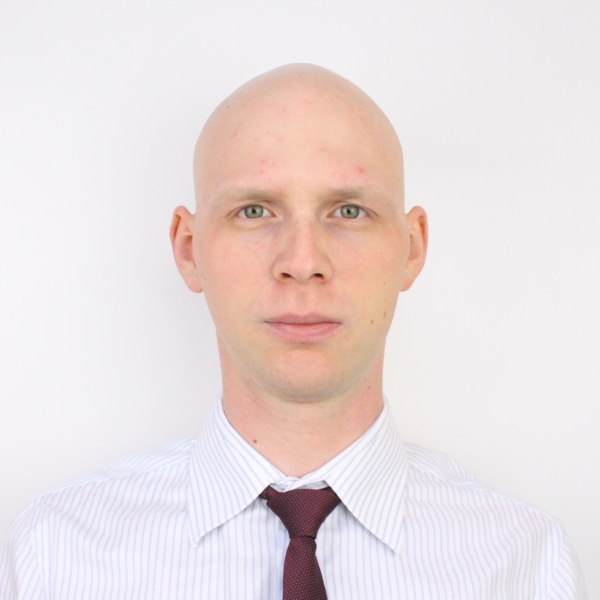
\includegraphics[width=0.2\textwidth]{portrait.jpeg}
    \captionsetup{labelformat=empty}
    \caption{Moscow, Russia \\ 
    1 Nov 1991 \\ 
    ipkharitonov@gmail.com \\
    \href{https://github.com/neer201}{github.com/neer201} \\
    \href{https://www.linkedin.com/in/ivan-kharitonov-34650/}{LinkedIn} \\
    +7(916)785-71-11 }
\end{SCfigure}
% 
%--------------------STATEMENT----------------------
I seek a research/software engineer position connected with deep learning. I am interested in self-driving and robotics areas and have some experience with it.

\section*{Education}
\begin{tabular}{@{}L!{\VRule}R}
    2008 -- 2014 & \textbf{MS + BS} (electrical engineering) at \textbf{Bauman Moscow State Technical University} \\
    % (Radioelectronic Systems and Devices - Radars) \\
    2016         & Data Mining in Action course (open ML course at MIPT)                                          \\
    2017 -- 2019 & \textbf{Yandex School of Data Analysis} -- Computer Science track    \\
    2019, 2021 & Summer school "Control, Information, Optimization" \\
    2020 & Waymo workshop for FSG Academy - \href{https://drive.google.com/file/d/1-WxECccxBrRWIvEt9WQeXKTueiF658r7/view?usp=sharing}{certificate} \\ 
    2021 & Third HSE-Yandex autumn school on generative models - \href{https://indico.cern.ch/event/1082512/timetable/#20211123}{info}\\
\end{tabular}
\section*{Teaching}
\vspace{-0.5em}
\begin{tabular}{@{}L!{\VRule}R}
    % YSDA
    spring 2019-2022                                                                                                                                         \\ {\boldgrey{Yandex DA school}} \\ &
    {\textsc{Teaching assistant for the course Practical RL}} Provided help and read seminars (model free methods and MCTS) with hw checkups in HSE and YSDA \\
\end{tabular}

\section*{Professional Experience}
\begin{tabular}{@{}L!{\VRule}R}
    % Sberautotech
    Aug 2020 -- now                                                                                                       \\ {\bf Sberbank} \\ \boldgrey{Sberautotech \\} &
    {\textsc{Software engineer - perception team}}

    \begin{itemize}
        \item Implemented models for point-cloud based object detection task.
    \end{itemize}
    
    \textsc{Software engineer - prediction team}
    \begin{itemize}
        \item Multi-object tracking -- solve object tracking problem using random finite set statistics.
    \end{itemize}                                                                                                  \\
    % 
    % FSUE NAMI
    Jul 2015 -- Nov 2017                                                                                                       \\ {\bf FSUE NAMI} \\ \boldgrey{Central Scientific Research Automotive Institute -- \\ Information and Intelligent Systems Center} &
    {\textsc{Research engineer at self-driving department (\href{https://www.engadget.com/2016/08/28/yandex-teams-on-self-driving-shuttle-bus/}{Shuttle project})}}
    % 
    \begin{itemize}
        \item Implemented perception models for object detection task -- collecting/generating training data, optimizing the model design, model implementation (Caffe DL framework) and evaluation.
    \end{itemize}
    \textsc{Software developer (Control systems) at transmission control systems department (\href{https://en.wikipedia.org/wiki/Aurus_Senat}{Aurus project})}
    \begin{itemize}
        \item System identification -- created plant models for some vehicle mechanism, such that gearbox clutch hydraulic actuator.
        \item Implemented basic software layer for automotive microcontroller (C, Simulink, Altium Designer) from scratch.
        \item Designed and implemented a controller for hydraulic actuators with further improving quality metrics and decreasing system setting time.
        \item Decreased calibration time by developing automated calibration procedure of control system parameters and tested control algorithms on the testbench.
    \end{itemize}                                                                                                  \\
    % 
    % FORMULA STUDENT
    Mar 2013 -- Aug 2015                                                                                                       \\ {\bf BMSTU \\ \boldgrey{Bauman Moscow State Technical University}} &
    {\textsc{Hardware and telemetry engineer on \href{https://baumanracing.ru/en/}{an FSAE team}.}}
    Participated in international engineering competition FSAE as a member of the university racing team.
    % 
    Responsibilities: hardware and software development, sponsorship and partnership management.
    % 
    Achievements:
    \begin{itemize}
        \item Released projects: MS thesis -- using RTK navigation for telemetry, F1-like steering wheel with integrated LCD, wireless telemetry module, signals expansion module by reverse-engineering the race ECU CANbus protocol.
        \item Received positive feedback from judges on the design event with good score.
        \item Established sponsorship contracts with several companies. As a result, we were granted new equipment.
    \end{itemize}                                                                                              \\
    % 
    % CRYPTO LLC
    Feb 2012 -- Jul 2013                                                                                                       \\ {\bf Crypto LLC \\ \boldgrey{Systems integrator}} &
    {\textsc{Engineer at System Integration Department.}}
    \begin{itemize}
        \item Adapted the product to the customer by adding fault tolerance setup.
        \item Integrated the monitoring tool (Zabbix) with a data management system.
    \end{itemize}                                                                                                  \\
    % 
    % Dominanta Vimpelcom
    May 2009 -- Feb 2012 {\bf PJSC VimpelCom} &
    {\textsc{Test Engineer.}} The Vimpelcom`s \href{https://www.dvb.org/news/russia-to-launch-dvb-h-services}{pilot project} - TV provider for mobile phones.
    \begin{itemize}
        \item Monitoring of the head and base stations (DVB-H) and 2nd level technical support.
    \end{itemize}
\end{tabular}
\section*{Generall Skills}
\begin{tabular}{@{}L!{\VRule}R}
    Programming    & Python (numpy, scipy, pytorch, jax, pytest, poetry, nox) \\
    & MATLAB, C++                    \\
    Tools &  CI/CD (github actions, gitlab-CI), ROS2, xpra, git, ssh, unix, latex , Docker, dvc \\
    Engineering tools &  Altium Designer, Solidworks, LabView, Simulink, Vector software (CANape) \\
    Speaking      & Russian -- Native, English -- B2                      \\
\end{tabular}
\section*{Activities}
\begin{tabular}{@{}L!{\VRule}R}
    
    Formula Student & {\textsc{design judge}} \href{https://www.imeche.org/events/formula-student/team-information/fs-ai}{FSAE AI UK} 2020 \\
                    & {\textsc{design judge bay chief}} Formula Student Russia 2020 \\
                    & {\textsc{design judge (driverless - perception)}} \href{https://www.formulastudent.de/fsg/}{Formula Student Germany} 2021 \\
                    & {\textsc{design judge bay chief}} Formula Student Russia 2021 \\ 
    Motorsport      & {\textsc{Flag Marshal}} 2020 Formula One Sochi Gran Prix , 2020 Russian Circuit Racing Series \\
                    & {\textsc{Scrutineering, data analysis}} 2021 Russian Circuit Racing Series \\
                    & {\textsc{Scrutineering}} 2021 Russian Hot Hatch Club Championship \\ 
                    & {\textsc{Scrutineering}} 2021 Formula One Sochi Gran Prix \\
    Sports   & road bicycle racing, boxing \\
    Other activities & organized reading club about robotics and self-driving at BMSTU
\end{tabular}
% 
\end{document}